\documentclass[letterpaper]{article}
\usepackage{natbib,alifeconf}
\usepackage{epstopdf}
\usepackage{amsmath}

\usepackage{color,soul} %to be removed before submission

\title{Evolution, development and learning with predictor neural networks}
\author{Konstantin Lakhman \and Mikhail Burtsev \\
\mbox{}\\
Neuromorphic Cognitive Systems Lab, Kurchatov NBICS-Centre, \\
National Research Center ``Kurchatov Institute'', 1 Kurchatov sqr., Moscow, Russia \\
klakhman@gmail.com}

\begin{document}
\maketitle

\begin{abstract}
	Predictor neural networks is an innovative model for self-learning.
\end{abstract}

\section{Introduction}
The problem of adaptation in multi-goal environments is a great challenge for state of the art machine learning. 

Artificial neural networks with unsupervised learning are suitable for automatic classification tasks but not sufficient for implementation of neurocontrollers for autonomous agents.

Supervised learning in neural networks can solve the problem of adaptation in theory but it requires data of all sensory inputs with corresponding desired actions for the task environment. For any practical situation obtaining full information of this kind is infeasible.

Reinforcement learning algorithms commonly apply to isolated problems.

Neuroevolution solves the problem in constant but is limited in stochastic or changing environments.

What is required for the neural network learning algorithm to adapt successfully in multi-goal environment? Starting from the theories of functional systems~\citep{Anokhin1974} and neuronal group selection~\citep{Edelman1993} we suggest the following logic to derive such requirements. The neural network should be able to produce initial or \textit{primary} repertoire of basic behaviors. When during lifetime the agent starts to encounter problems in achieving goals with the primary behaviors then this initial repertoire should be extended to allow mission completion for a spectrum of environmental variations. These particular solutions acquired by learning constitute the \textit{secondary} repertoire of behaviors. Primary behaviors can be generated by evolutionary and developmental algorithms or pre-specified by hand. During life-time adaptation learning algorithm should detect failures to execute existing behaviors and generate actions to create alternative solution. We suggest that failure detection should be distributed over the whole neural network. Our hypothesis is that such prediction is possible when neurons not only activate but also predict future activity of each other. If some neurons detect mismatch between predicted and actual activities then the learning starts. We require that creation of a new action sequence should not disrupt existing behavior. This can be achieved by integration of new neurons in the network during learning process without changing already existing part of the network. The key feature of our model that makes adaptive learning possible is distributed prediction on the level of individual neurons, so we call this architecture \textit{predictor neural network}. In this paper we present computational study of the model consisting of evolutionary and developmental phases for generation of primary behavioral repertoire as well as life-time phase with learning controlled by continuous distributed prediction on the neuronal level. %(Fig.~\ref{Model_Overview}).

%\begin{figure}[b!]
%	\begin{center}
%	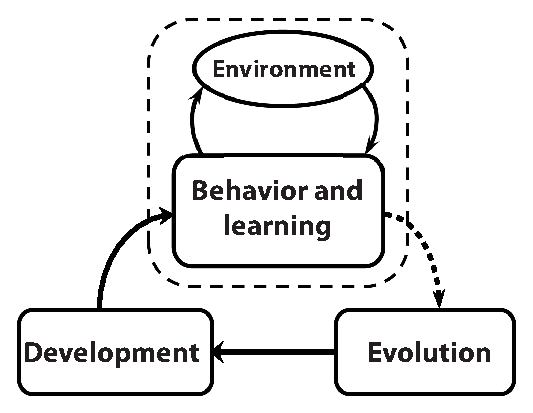
\includegraphics[width=6cm]{Fig1_Model_Overview.eps}
%	%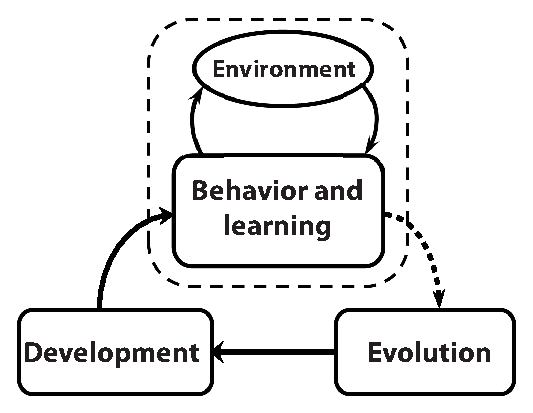
\epsfig{file=Fig1_Model_Overview.eps, width=8.4cm}
%	\caption{Schematic representation of the model's components}
%	\label{Model_Overview}
%	\end{center}
%\end{figure}

\section{The Model}

\subsection{Overview}

According to the neuronal group selection theory~\citep{Edelman1993} developmental algorithm in our model targets two different objectives: 1) generation of a primary repertoire of behaviors and 2) generation of {\em ``diversity of repertoires''} required for further self-learning during the life. During development an agent's genotype translates into the neural network controlling the agent's behavior in the environment. Diversity required for the selection of neuronal groups is implemented by simulation of the brain's anatomical regions with \textit{neuronal pools}. Neurons in the same pool have similar but not identical connections with the rest of the network. During development endogenous stochastic activations of neurons lead to selection of highly connected subnetworks. These subnetworks produce primary behaviors of the agent. Remaining neurons form a set of {\em silent neurons} that are used for learning.     

In the theory of functional systems~\citep{Anokhin1974} every goal-directed behavior serving some adaptive function unfolds in three stages: 1) generation of an action and prediction of its' results; 2) evaluation of results after action completion; 3) formation of a new functional system of neurons if additional leaning is needed. To implement both generation of action and evaluation of results neurons in our model have two types of synapses namely \textit{effector} and {\em predictor}. Effector synapse is the same as in the standard artificial neural network. Predictor synapse does not propagate excitation but contributes to prediction of future activity of the neuron. Moments of the {\em mismatch} between expected results and state of the environment are detected in the neurocontroller as neurons calculate discrepancy between predicted and observed activity of each other. detected mismatch initiates activation of silent neurons to modify agent's behavior. Agent's ability to generate meaningful and useful predictions at the neuronal level is subject to evolutionary selection of predictor connections in the network.

\subsection{Multi-goal Environment and Neural Net}

In the model population of agents evolves on the hypercube. State of the environment is represented by a binary string and at each discrete time step the agent can change the state of one bit. A goal in this environment is defined as the consecutive changes of a particular bits of the state vector. Set of such a goals in the environment forms a branched hierarchy. One goal could be nested in another one, i.e. be a beginning of it, and different goals could have identical starting nested goal. Detailed description of the environment can be found in ~\citep{LakhmanBurtsev2013}.

The agent operates in the environment for a fixed amount of time. Fixed reward is associated with each goal and a value of reward accumulated over life-time affects the reproductive success of an agent at the evolutionary phase of the simulation. However, in contrast to the paper~\citep{LakhmanBurtsev2013} we have changed how reward is recovered in the case when the agent attempts to reach the same goal during its' recovery period. Previously, the reward associated was reseted to zero on the goal's completion and then linearly recovered to the initial value. The agent had no information about accumulated reward. As we introduce learning in the current study there should be some feedback from the environment to the agent that completion of the goal failed. In the current version of the model completion of the goal during value recovery is impossible. If the agent tries to perform an action that would lead to the finalizing of the goal with the value of reward smaller than initial then the change of the bit is blocked and the state vector of the environment remained the same. Thus, the agent can perceive failure to complete target action sequence by the neurons predicting the environmental change after successful action. Note that in the current scheme of agent-environment interaction the agent also has no direct information about the value of reward.

 The structure of the agent's neurocontroller is determined by a processes of evolution, development and learning. The controller consists of three sets of neurons: input, output and interneurons. Number of input and output neurons is fixed and determined by a dimension $n^{\mathrm{env}}$ of the hypercube ($n=8$ for all simulations). Input neurons represent current state vector with one neuron for each bit. Output neurons encode action that agent performs on a current time step. Each pair of output neurons is responsible for turning on or off a particular bit of the state vector. Current agent's action are selected according to the pair of the most active output neurons. 
 
% Thus, the number of output neurons is determined as:
%\begin{equation}
%	n^{out}=\underset{n}{\operatorname{argmin}} \left[\dbinom{2}{n}\geq2n^{env}\right] \enspace . 
%\end{equation}   

Interneurons of a neurocontroller are organized in layers with no restriction on connectivity. This allows to form both direct and recurrent effector synapses. Recurrent effector synapses receive excitation with a unit time delay.

\subsection{Evolutionary Algorithm}

Genotype of an agent is defined by a tuple:

\begin{equation}
	G = \left( P, EC, PC\right)\enspace, 
\end{equation} 

\noindent where 
$P = \left\{P_{\alpha}\right\}$ is a set of neuronal pools, 
$EC = \left\{ec_{\gamma\alpha}\right\}$ is a set of effector connections between pools, 
$PC = \left\{pc_{\gamma\alpha}\right\}$ is a set of predictor connections. 
During development this genotype is translated to the neural network. Each neuronal pool $P_{\alpha}$ of the genotype corresponds to a group of neurons with similar connectivity topology and has the following parameters: pool's size $c_{\alpha}$, i.e. the number of neurons that will be formed from this pool during development; mean $m_{\alpha}$ and standard deviation $\sigma_{\alpha}$ of the biases of the neurons, that corresponds to a particular pool.

Each effector connection $ec_{\gamma\alpha}$ between pools $\alpha$ and $\gamma$ has the following parameters: mean $m_{\gamma\alpha}$ and standard deviation $\sigma_{\gamma\alpha}$ of the weights of the synapses, that will be formed between neurons belonging to the corresponding pools; probability of the synapse development $p^{\mathrm{dev}}\left(ec_{\gamma\alpha}\right)$.

The only parameter for predictor connections $pc_{\gamma\alpha}$ is probability of connection development $p^{\mathrm{dev}}\left(pc_{\gamma\alpha}\right)$.

Reproductive success of the agent, i.e. the probability to be selected as a parent for the next population, is directly proportional to the value of reward accumulated over fixed amount of time. An offspring inherits parent's genotype transformed by mutations, including all numerical parameters of the genome introduced above. The structure of the network is modified by {\em duplication pool} mutation described in detail in the paper~\citep{LakhmanBurtsev2013}. This mutation substitute a single ``parent'' pool with two ``offspring'' pools with the same connectivity structure and half the size of the ancestor. We also used addition and deletion of effector and predictor connections as additional structural mutations. Full list of values of parameters that have been used for the simulations is provided in the Appendix A.

\subsection{Developmental Algorithm}

\subsubsection{Generation of neuronal pools} Development starts with translation of the agent's genotype $G = \left( P, EC, PC\right)$ into complete network. Each neuronal pool $P_{\alpha}$ is filled with $c_{\alpha}$ neurons. Bias $b_{i}$ for the neuron $v_{i}$ is drawn from a normal distribution: $b_{i}\sim \mathcal{N} \left(m_{\alpha},\sigma^2_{\alpha}\right), \enspace \forall v_{i} \in P_{\alpha}$. Effector synapse is created between neurons $v_{i} \in P_{\alpha}$ and  $v_{j}\in P_{\beta}$  according to the pool connectivity coded in the genome: $ w_{ji} \sim \mathcal{N} \left(m_{\beta\alpha},\sigma^2_{\beta\alpha}\right)\enspace \mbox{with probability} \enspace p^{\mathrm{dev}}\left(ec_{\beta\alpha}\right),\enspace \mbox{if} \enspace ec_{\beta\alpha} \in EC ; \mbox{and} \enspace w_{ji} = 0$ otherwise (the synapse is not developing). As a result every neuron in the net has unique connectivity structure both in terms of topology and weights distribution. Development of predictor synapses occurs similarly with the only exception that predictor synapse has no weight.

Similar model of neuroevolution with pools encoded in the genome was  proposed in the framework of {\em Enforced Sub-Populations} evolutionary algorithm~\citep{GomezMiikkulainen1999}. \hl{However, according to this algorithm only one neuron was selected from each pool in the development.  In this case, this mechanism was used to decrease the co-adaptation of different neurons, that lead to development of unique specializations of neurons. \textbf{MB: cant understand this}}

\subsubsection{Selection of primary neuronal groups} The next phase of neurocontroller development has a goal to select neuronal groups for the primary behavioral repertoire. To perform this developmental selection we utilize competitive principle proposed in the theory of neuronal group selection~\citep{Edelman1993} which states that neuronal groups with highest endogenous stochastic activity are selected. As a result network of active neurons constitute  neurocontroller at the beginning of agent's life. Less active neurons became silent but can be recruited later in the process of learning.

Selection of primary neuronal groups takes place in the isolation from the model environment for a fixed number of time steps $T^{\mathrm{sys}}$. At each time step each neuron of the network produces spontaneous activation with probability $p^{\mathrm{spon}}$. Outputs of the remaining neurons are calculated in the standard way using truncated positive sigmoid activation function (truncation implies zero output in case of the negative neuron's potential). Spontaneous activations of the neurons are designed to provide signal flow in the network in the absence of information about external environment. Total signed value of activation potential received by each neuron is calculated during simulation of endogenous network activity. Within each pool fraction $p^{\mathrm{act}}$ of the neurons is selected to participate in primary neuronal groups and remaining neurons become silent. The probability for the neuron to be selected is directly proportional to the corresponding value of accumulated potential.

The role of predictor synapses in the network is prediction of future activations of a neuron. If there is a predictor synapse between neurons $v_{i}$ and $v_{j}$ then pre-synaptic neuron's activity predicts that post-synaptic neuron will be active on the next time step (and vice versa in case of absence of activity). During development the predictor synapses between active neurons with prediction rate less then some threshold value $L^{\mathrm{sig}}$ ($0.5$ in the current study) are being deleted from the network. Predictor synapses connecting silent neurons remained intact. 

It should be noted that the outputs of silent neurons during the agent's life are always set to zero, regardless of the value of potential they receive by incoming effector synapses.     

\subsection{Learning Algorithm} 

Innate behavior produced by initial neural network right after development is not optimal and should be complemented by learning.

It is necessary to answer two basic questions when designing a learning algorithm: {\em 1)} when should learning begin?; {\em 2)} how to perform learning if it is needed. 

\subsubsection{Mismatch detection} To solve the first problem it is necessary to introduce mechanism for detection of the moments in which additional learning is needed. These are the moments when the agent performs actions that earlier led to adaptive result but now failed. Theory of functional systems~\citep{Anokhin1974} solves this problem by postulating that at the beginning of goal-directed behavior {\em functional system} of neurons (neural subnetwork responsible for some adaptive function) generates both the program of actions and prediction of expected outcomes so-called {\em acceptor of action results} (AAR). If AAR is not consistent with observed features of the environment, obtained immediately after the performance of the planned action, then functional system enters so-called {\em mismatch state} and initiates learning. \hl{Functional systems interact with an environment as well as with other functional systems. \textbf{MB: there is no explicitly stated interactions between FSs in classic TFS}} In our model predictor synapses make possible distributed evaluation of goal-directed behavior on the level of individual neurons. Several theoretical papers concluded that the biological neurons are able to provide similar functions~\citep{Fiorillo2008}.

Let consider single neuron as a functional system. Signals from other neurons constitute its' ``environment''. At a given time step the neuron can be excited or nonactive. 
In the model the neuron is in the excited state when its output is greater than zero. 
Each neuron forms prediction about its own future activity based on predictor synapses from other neurons. 
\hl{Each presynaptic neuron makes its contribution to the total prediction in accordance with the following scheme: if the presynaptic neuron was excited at time step $t$ then it predicts that the postsynaptic neuron will be excited at time step $t+1$, and vice-versa if the presynaptic neuron was in the ground state.}
Thereby each neuron could calculate probability distribution of its own activity on the next time step based on predictor signals:

\begin{equation}
	\label{eq3}
	\begin{array}{c}
		p^{\mathrm{exc}}\left(v_{j}, t\right) = \frac{\left\vert\left\{v_{i} | \ ps_{ji} \in PS,\ o_{i}\left(t-1\right)>0\right\}\right\vert}
			{\left\vert PS_{j}^{\mathrm{act}}\right\vert} \\
			\\
		p^{\mathrm{sil}}\left(v_{j}, t\right) = 1 - p^{\mathrm{sil}}\left(v_{j}, t\right)
	\end{array}
	\enspace , 
\end{equation}      

\noindent where $p^{\mathrm{exc}}\left(v_{j}, t\right)$ is the probability of neuron $v_{j}$ of being active at time step $t$, $PS$ is a set of network's predictor synapses, $o_{i}$ is the output of neuron $v_{i}$, $PS_{j}^{\mathrm{act}}$ is a set of incoming predictor synapses of neuron $v_{j}$ that are coming from active neurons. Neuron makes prediction based on this distribution only if one of these probabilities exceeds a fixed threshold $L^{\mathrm{pred}}\in\left(0.5,1\right]$.  Eq.~\ref{eq3} implies that only active neurons affect prediction. 

Described procedure assumes two types of the possible mismatch situations: I-type mismatch implies the absence of the neuron's activity when it was predicted and II-type mismatch implies the presence of the activity when it was not predicted. 

\subsubsection{Learning via activation of ``silent'' neurons} According to the systems-selection theory~\citep{Shvyrkov1986} learning at the neuronal level consists of neuronal specializations for the problem situation. This  specialization occurs via selection of neurons from the ``reserve'' of low active cells or, in our case, from silent neurons. 

Mismatch detection on the level of neurons allows effectively locate a specific place in a neural net where it is necessary to make modifications during learning. Thus for each neuron with I-type mismatch a silent neuron from the same pool with highest effector input is found and added to the set of network's active neurons. This just activated neuron is \textit{specialized} on solving current problem. Effector synapses of this neuron are pruned to maximize recognition of the current neuronal input. This implies deletion of effector synapses from neurons that have not been active on the current time step. Additionally we add a strong excitatory synapse $w\sim\mathcal{U}\left(0.5,1\right)$ from activated neuron to the mismatched one. This synapse could potentially lead to the elimination of the mismatch on the postsynaptic neuron in the similar behavioral situations in the future. We also add additional predictor synapses from the neurons that predicted activation of the mismatched neuron to the set of \hl{(incoming $-???->$ effector)} synapses of the activated neuron. 

Learning for the II-type mismatch occurs in exactly the same manner except that we add strong inhibitory connection from activated to mismatched neuron in order to avoid mismatch in the similar behavioral situations.   

As a result of learning the initial neural network is expanded by distributed integration of neurons specialized on solution of the current problem. This scheme fits into the conceptual framework considering learning as following the same principles as evolutionary process: generation of diversity and selection~\citep{Burtsev2008,burtsev2012adaptive}. The specialization of the silent neurons could be interpreted as a local mutations of neurocontroller, which can potentially lead to successful behavior. Nonetheless, learning terminates only if there is no mismatch between organism's expectations and actual state of environment detected at the neuronal level.      

\section{Experimental Results}

\begin{figure}[!b]
	\begin{center}
	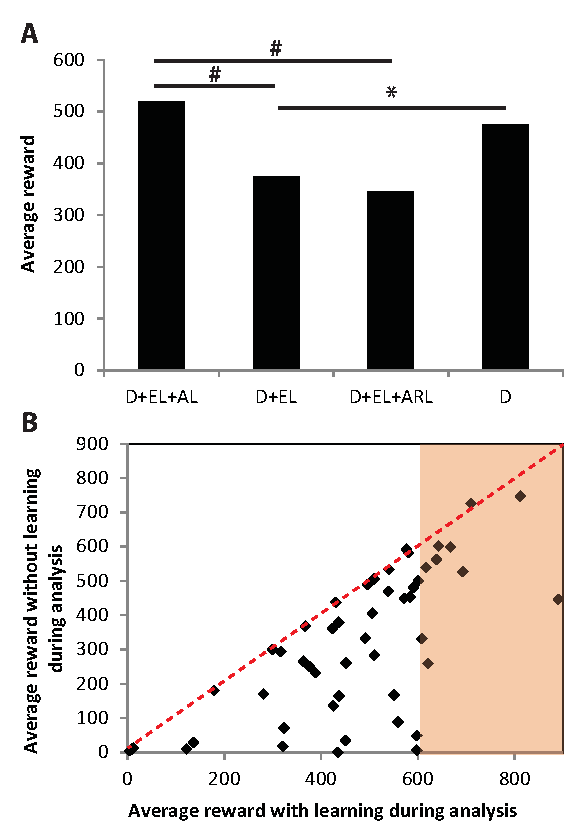
\includegraphics[width=8cm]{Fig2_Efficiency_analysis.eps}
	%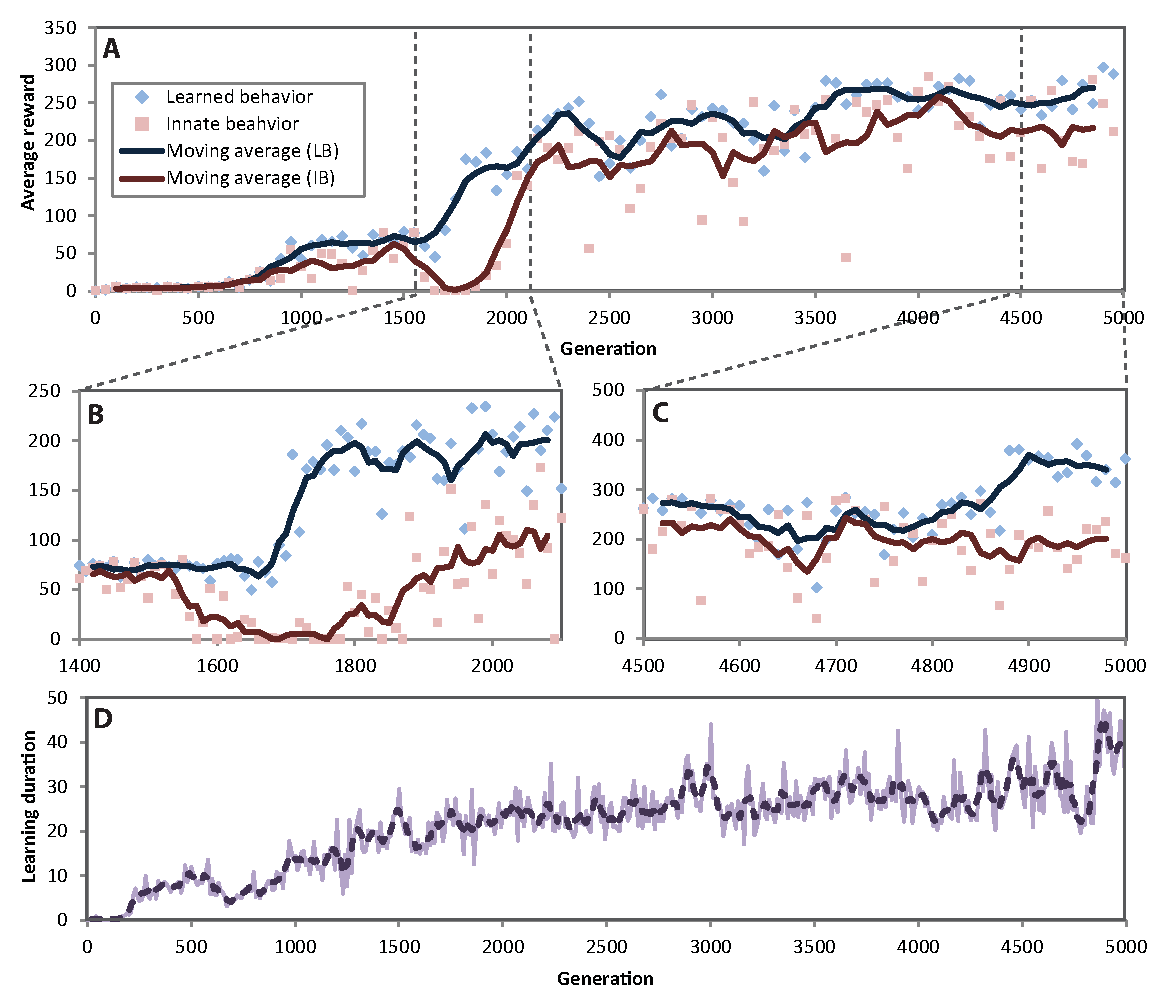
\epsfig{file=Fig3_Behavior_Evolution.eps, width=17cm}
	\caption{Effects of developmental and learning components of the model on reward. \textbf{A)} Average reward for the different types of agents (D -- development, EL -- learning during evolution, AL -- learning during an analysis phase, ARL -- ``random learning'' during an analysis phase). $\#$ denotes paired samples t-test with $p\mathrm{-value}<0.001$, $*$ denotes t-test with $p\mathrm{-value}=0.012$. \textbf{B)} Comparison of the efficiency of the same agents with and  without learning. Each dot represents averaged value for the best population of corresponding evolutionary run. The range of reward values of the best $20$ runs is highlighted.}
	\label{Efficiency_analysis}
	\end{center}
\end{figure}

\begin{figure*}[!t]
	\begin{center}
	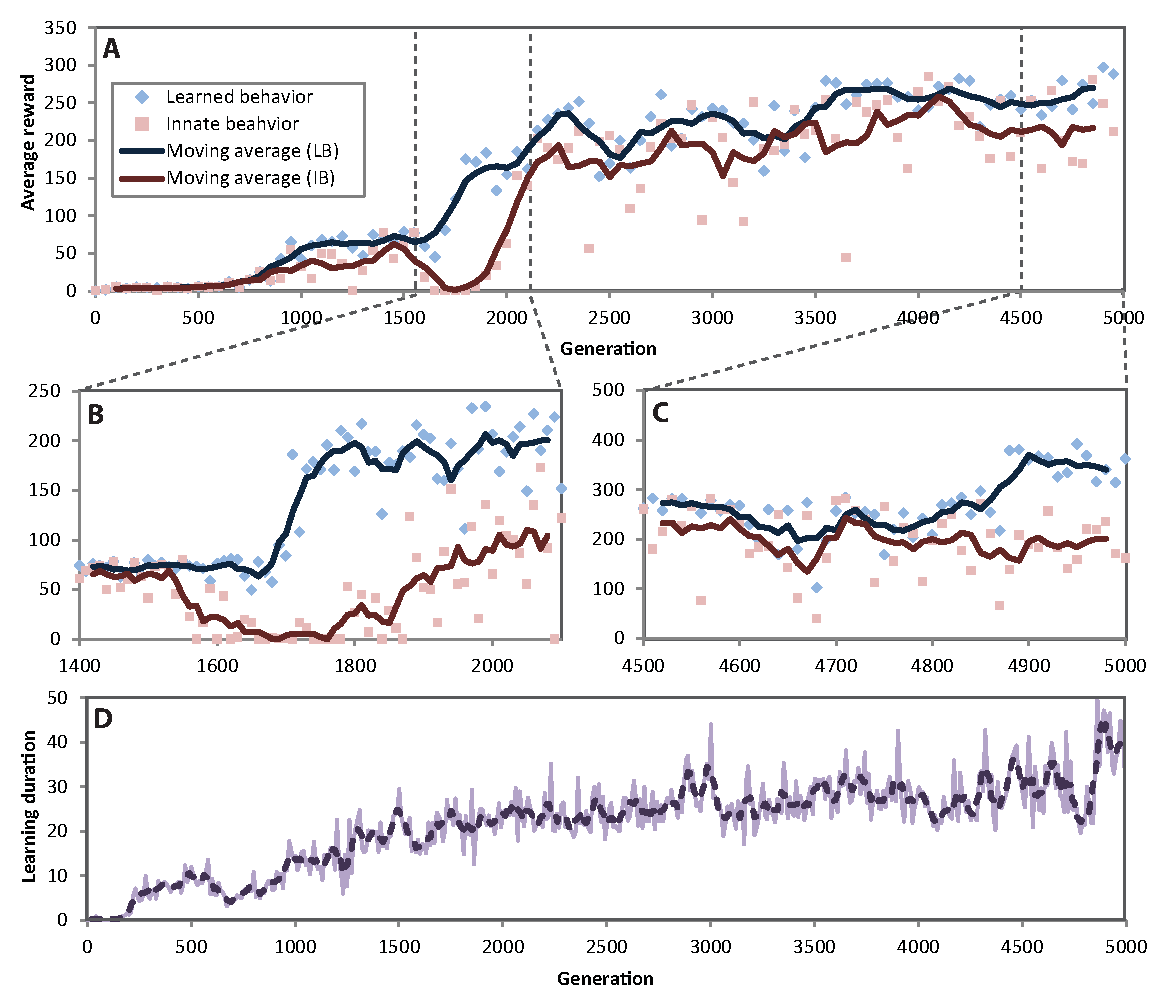
\includegraphics[width=16cm]{Fig3_Behavior_Evolution.eps}
	%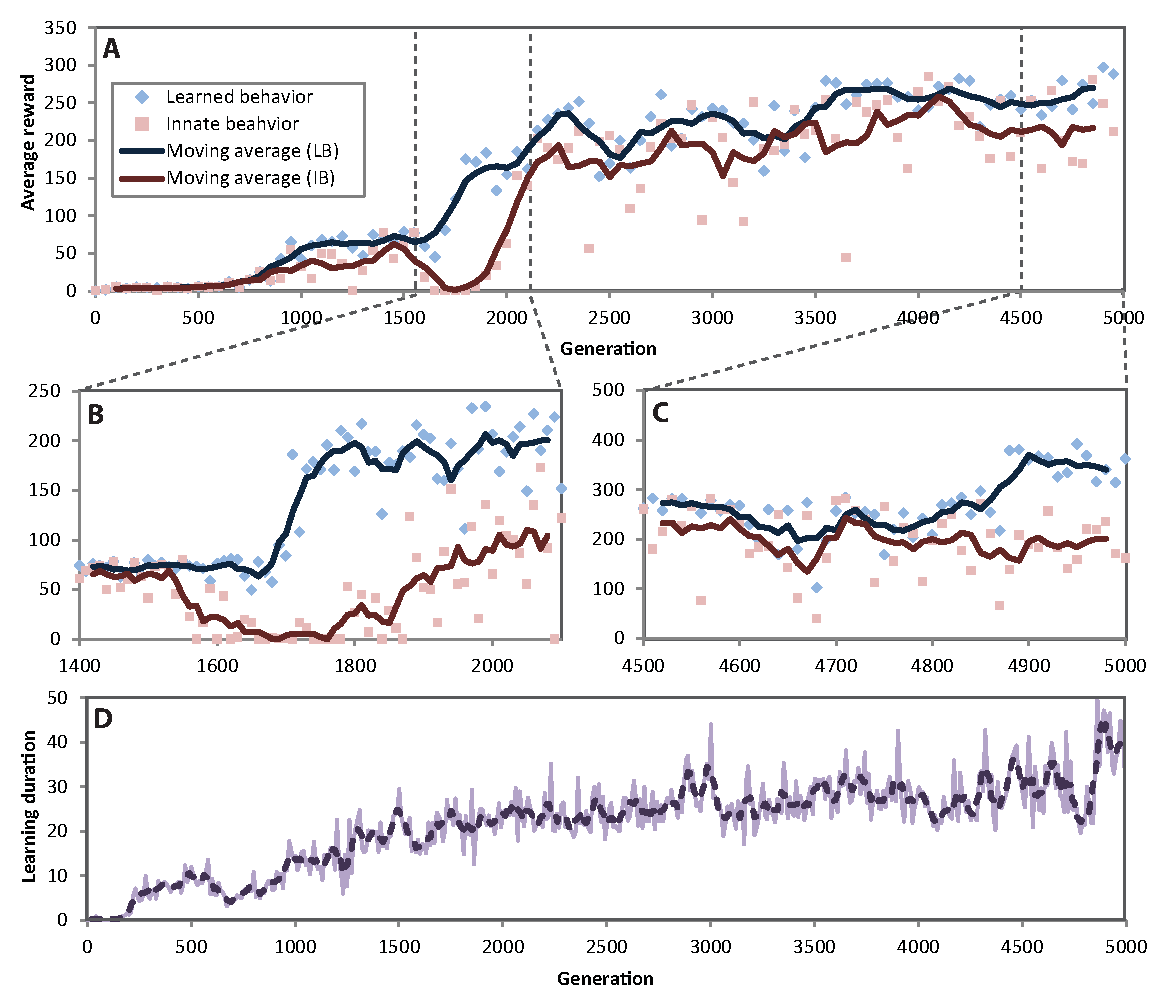
\epsfig{file=Fig3_Behavior_Evolution.eps, width=17cm}
	\caption{Evolutionary dynamics of innate and learned behaviors. \textbf{A)} Dynamics of the average rewards for the innate (pink) and learned (blue) behaviors for \hl{the best evolutionary run \textbf{MB: why avrg reward at the end of the best run is lower than avrg over all runs (fig 1A)?}}. The values are calculated for the best agent of the each $50$-th generation. \textbf{B-C)} Periods when average reward after learning increases. The values are calculated for the best agent of the each $10$-th generation. \textbf{D)} Averaged duration of learning. Duration of learning is calculated as the last time step of the agent's life when silent neurons specialize.}
	\label{Behavior_Evolution}
	\end{center}
\end{figure*}

As the first step we have studied how learning algorithm affects efficiency of an agents in terms of accumulated reward. 10 environments with different goals structure were generated randomly. Two modifications of the model -- with or without learning (only with developmental phase) were run in every environment 5 times (100 runs in total). Then we detected the best population in terms of the average accumulated reward in each run. For all agents in the best population development was performed 5 times with different random seeds. Finally, we run these 5 different controllers from all $2^{n^{\mathrm{env}}}=2^8=256$ initial states of the environment. Resulting values of average reward are shown on the Fig.~\ref{Efficiency_analysis}A. We have not found statistical difference between efficiency of the agents evolved with and without learning -- t-test showed $p\mathrm{-value}=0.23$. However, if learning is switched off for the agents evolved with it then average reward decreases significantly indicating importance of learning in this case.  Effect of learning is detailed on the Fig.~\ref{Efficiency_analysis}B where majority of runs show lower reward without learning.  

We have also tested our learning mechanism against simple random activation of silent neurons (Fig.~\ref{Efficiency_analysis}A). Random learning implies that silent neuron has a fixed probability of integration into the network at a given time step. We randomized learning of the agents evolved with learning. Several activation probabilities were examined from the interval $\left[0.01,0.1\right]$, but results are presented only for the best value of $0.5$. Random specialization of neurons do not increase reward compared to normal learning  and even get less reward than the same agents without any learning.

Results suggest that evolutionary algorithm alone is able to make non-learning agents almost as effective as learning ones. We found that after evolution the non-learning agents have in the neural net more pools and smaller pool sizes compared to the agents with learning (data is not shown). Larger pool sizes of learning agents indicate that selection support mechanism for variation of neuronal groups during learning. 

As the next step we have studied evolution of \hl{the best run \textbf{???}} in more details.
For the best agent of each generation 5 different phenotypes were produced by randomly initialized development and then tested with and without learning. Resulting dynamics of innate and learned behaviors are presented on the Fig.~\ref{Behavior_Evolution}A. Over the period of evolution an efficiency of learned behavior usually grows first and innate behavior follows.The increase of the best agent's reward after learning can occur both while efficiency of the innate behavior is decreasing (Fig.~\ref{Behavior_Evolution}B) or remains unchanged (Fig.~\ref{Behavior_Evolution}C). 

As we have showed earlier~\citep{LakhmanBurtsev2013} behavior evolved in the similar hypercubic environment consists of two phases: convergence phase when the sequence of actions depends on the particular initial state and stable repeating cycle of actions. We will call the latter behavioral cycle. Analysis of behavior cycles evolution for the best run shows that significant growth of learning efficiency is accompanied by explosion in variability (up to $200$ variations) of behavioral cycles and subsequent change of the dominant behavioral strategy (data is not shown). The number of observed behaviors are sharply reduced when we analyze the same agents but without learning. This might represent a general scenario when learning guide evolution of complex adaptive behavior in natural and artificial systems. 

Reward accumulated by the agent during learning sometimes increases together with the average learning time, i.e. the period of silent neurons specialization(for example, starting from $4850$-th generation on the Fig.~\ref{Behavior_Evolution}D). Dynamics of the specialization of silent neurons during the learning process averaged over the best $10$ evolutionary runs is shown on the Fig.~\ref{Activations_dynamics}. On the average about $50\%$ of all silent neurons are turned on lifelong, but most of them are specialized at the beginning of life (up to $10$-th time step). However, sometimes learning takes place even as late as $100$-th time step for some of the evolutionary runs.  

\begin{figure} %[!b]
	\begin{center}
	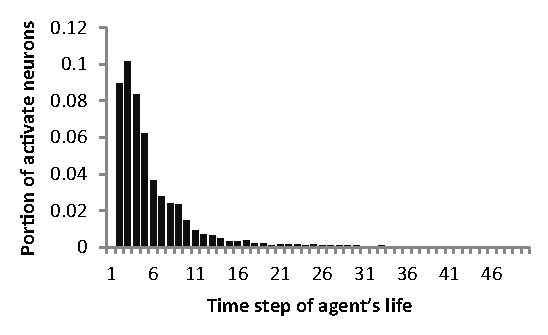
\includegraphics[width=8cm]{Fig4.eps}
	%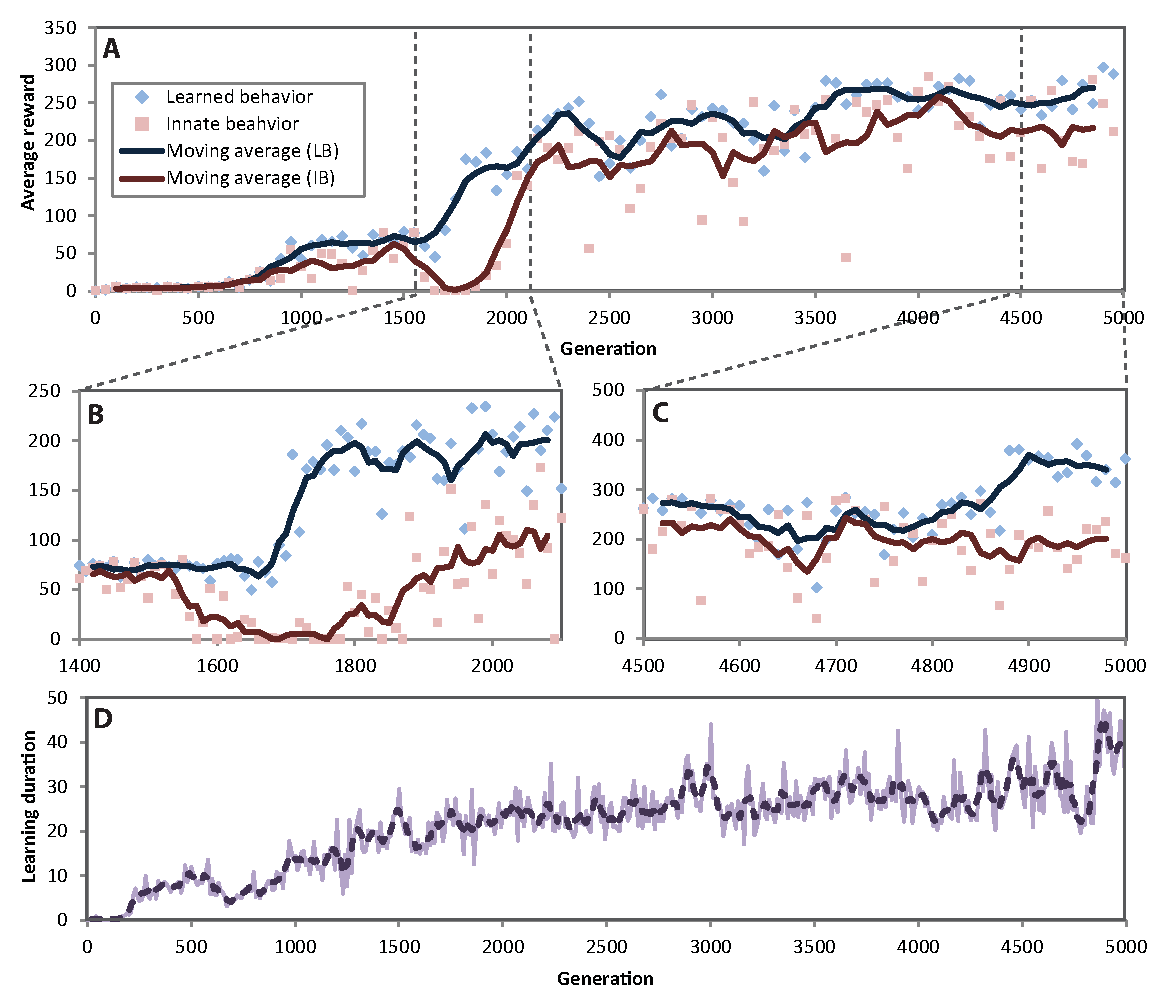
\epsfig{file=Fig3_Behavior_Evolution.eps, width=17cm}
	\caption{Timing of silent neurons specialization during an agent's life (averaged over the best $10$ evolutionary runs).}
	\label{Activations_dynamics}
	\end{center}
\end{figure}

We found that there are the periods of evolution when success of learning significantly correlates with the number of specialized silent neurons (Fig.~\ref{Neurons_Learning_Correlation}). This happens when behavior of the agents is not fully formed \textbf{\hl{(??? or the dominant strategy changing)}} and learning can play significant role in improvement of partial action sequences. Later in the course of evolution (for example in the $3500$-th generation on the Fig.~\ref{Behavior_Evolution}) this correlation disappears and roughly the same number of silent neurons are being activated regardless of the difference between learned and innate behavior (data is not shown). It seems that the role of learning is changing here, it mainly ``corrects errors'' that were made in the developmental process. On this stage the development can generate neurocontrollers that accumulate the same reward with or without learning. 

\begin{figure} %[!b]
	\begin{center}
	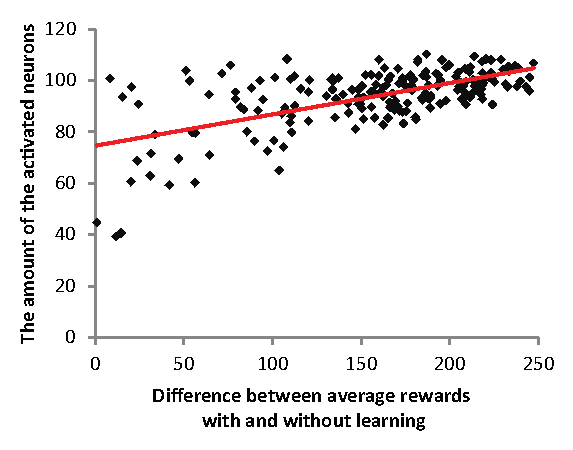
\includegraphics[width=8cm]{Fig5.eps}
	%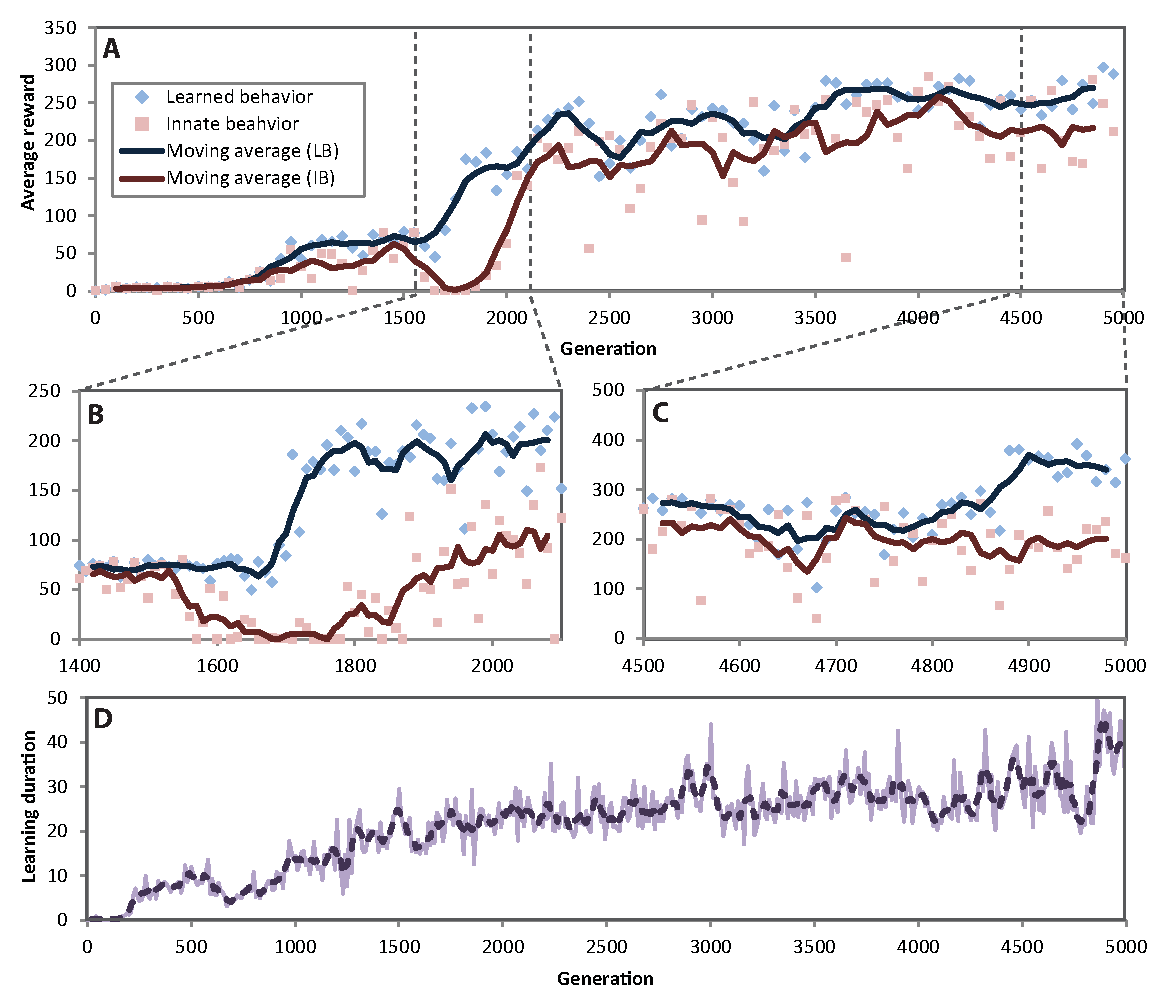
\epsfig{file=Fig3_Behavior_Evolution.eps, width=17cm}
	\caption{The number of activated silent neurons positively correlate with the quality of learning. Each point represents value of reward averaged over all initial states of the environment for one development of the best agent of $1781$-th generation from the Fig.~\ref{Behavior_Evolution}. Spearman correlation coefficient $\rho=0.52$ with $p\mathrm{-value}<0.001$}
	\label{Neurons_Learning_Correlation}
	\end{center}
\end{figure}

To investigate how the neural network can generalize after learning we put the agent in each one of the states of the environment to learn then this agent with neural net after learning was tested starting from all the other states (Fig.~\ref{Learning_Process}A). For this we have chosen the agent from the later stage of evolution (the best agent of $4950$-th generation) with the big difference between rewards with and without learning. Fig.~\ref{Learning_Process}A demonstrates that the neurocontroller after learning from one state of the environment is also efficient in the most cases  when the agent starts life from the different state. ``Stripes'' on the figure correspond to the sets of initial states with different accumulated reward for the same neural net. This means that the agent achieves the same goals in the same order, but can be more or less optimal in terms of the number of actions performed. 

The same agent that was used to produce Fig.~\ref{Learning_Process}A was utilized to study dynamics of the learning process (Fig.~\ref{Learning_Process}B). The agent was started with learning from a few states and then after each time step we evaluated efficiency of the controller, obtained so far, by running its non-learning version from all states of the environment. The results demonstrate that  learning occurs only at the earliest stage of agent's life during the first 6--10 time steps. This is also consistent with the average dynamics of the specialization of silent neurons presented on the Fig.~\ref{Activations_dynamics}. Important feature of the learning process is that it is non gradual. Learning can even lead to temporary degradation of the intermediate controller performance. However then learning is finished the agent behavior abruptly becomes adaptive.

\begin{figure*} [!t]
	\begin{center}
	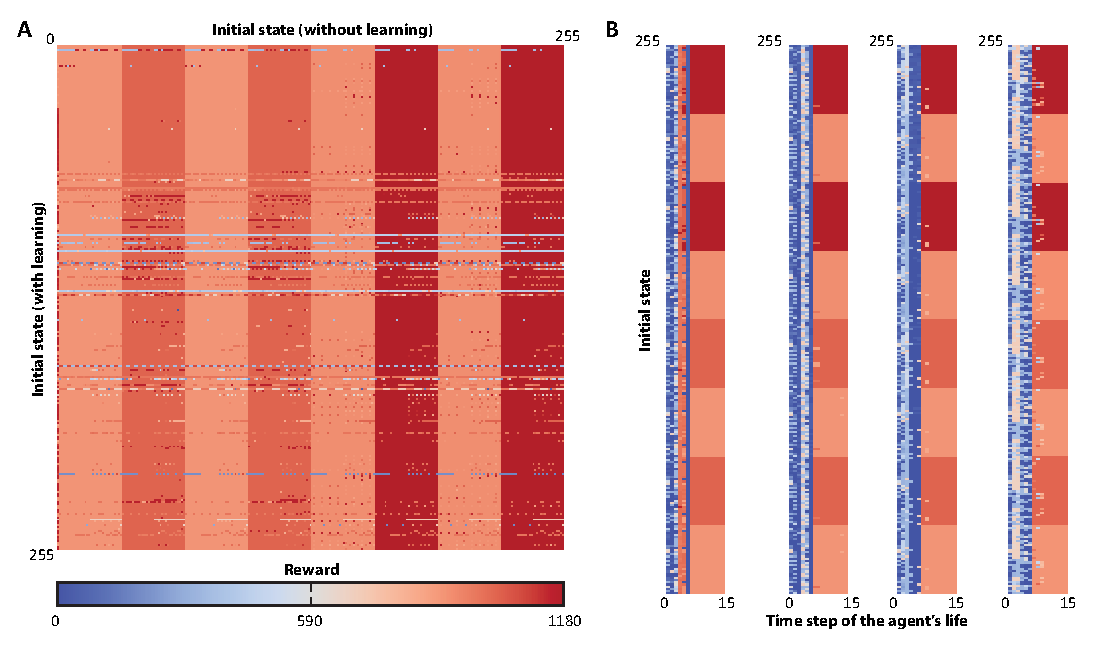
\includegraphics[width=16cm]{Fig6.eps}
	%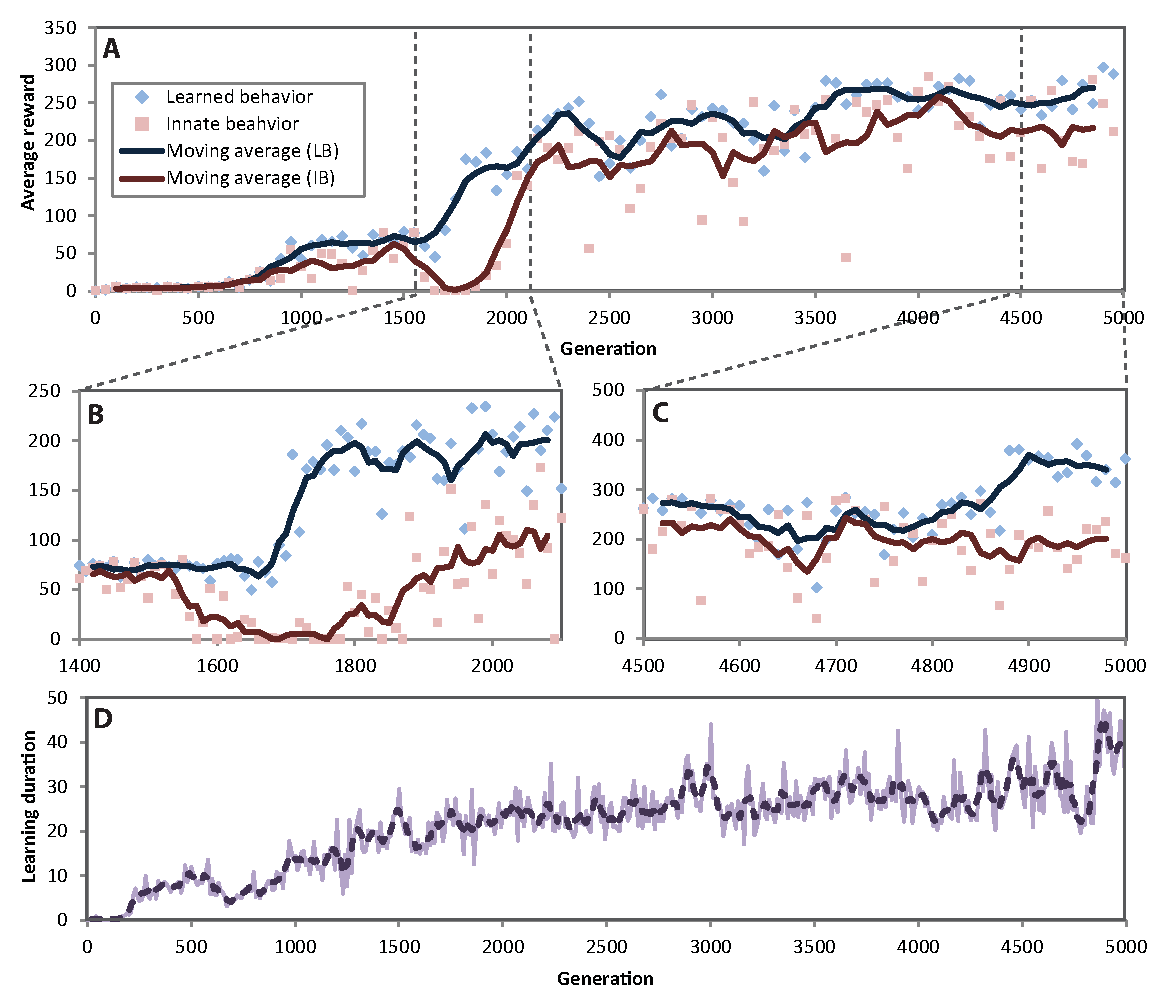
\epsfig{file=Fig3_Behavior_Evolution.eps, width=17cm}
	\caption{Neurocontroller performance after learning. \textbf{A)} After learning from each state of the environment the same learned neural network was started from each other state with the learning turned off. \textbf{B)} Performance of neurocontroller on the different stages of learning (see text for the details). 
	All results presented on the figure are for the best agent of the $4950$-th generation from the Fig.~\ref{Behavior_Evolution}(see text for more details).}
	\label{Learning_Process}
	\end{center}
\end{figure*}

\section{Conclusions}

\footnotesize
\bibliographystyle{apalike}
\bibliography{ALIFE14_paper}

\end{document}
